\documentclass{homework}
% \usepackage{graphicx} % Required for inserting images
\usepackage{amsmath}
\usepackage{gensymb}
\usepackage{subfig}
\usepackage{float}

\class{ECEN 5407}
\title{Homework 5}
\author{Sean Jennings}
\date{November 29, 2023}

\begin{document}
\maketitle

\section{Storage Systems}

\begin{letterenum}
    \item The following are grid storage technologies:
    \begin{enumerate}
        \item Battery Energy Storage (BES)
        \item Hydrogen gas
        \item Compressed Air Energy Storage (CAES)
        \item Pumped Hydropower
        \item Thermal Energy Storage
    \end{enumerate}

    Battery energy storage is a broad category of technologies which store
    energy in an electrochemical form. Specific types of batteries include:
    \begin{enumerate}
        \item lithium Ion batteries,
        \item lead acid batteries,
        \item Sodium Ion battieries,
        \item Flow batteries
        \item Flywheels
        \item Super capacitors
    \end{enumerate}

    Types of grid services that can be provided include:
    \begin{enumerate}
        \item Peak Shaving (reducing peak load)
        \item Energy shifting/arbitrage (storing power when energy is cheap/plentiful,
            discharging when it is expensive/load is high)
        \item Frequency Regulation
        \item Distribution/Transmission System upgrade defferals
        \item Renewable Capacity firming (allow interrmitent renewables to operate
            more efficiently; reduce curtailment)
        \item Interseasonal storage
        \item Operating (e.g. spinning) reserves
    \end{enumerate}

    Which of these grid services each of storage technology can provide
    is typically related to the ratio between power and energy capacity
    (in other words, the storage duration)
    for an economically efficient deployment of that technology, as well
    as its response time.

    For example, the cost of a hydrogen storage system is
    comparatively less for when storage container is sized for large durations.
    making it a better choice for interseasonal storage. CAES is similarly
    more economic at longer durations. These would be less suitable for
    shorter timescale services such as frequency regulation.

    On the other hand, batteries (particularly Li) have a very fast response time,
    making them suitable for frequency regulation applications.

    Thermal Energy (i.e. molten salt) energy storage is often integrated with
    concentrated solar power plants to that generation can be shifted to the
    time from daylight hours when solar power is high to evening hours
    when load is higher. This could be considered both an energy shifting
    and a renewable capacity firming application.

    Pumped hydro was traditionally built to supplement nuclear plants
    which run more or less continuously. This is an energy shifting/arbitrage
    service. 

    Flywheels and super capacitors has very short energy storage durations and 
    are typically used to provide frequency and power quality services, and
    would not be suitable for longer-term energy arbitrage.

    We note that there's quite a bit of overlap between these various grid
    services that can be provided and it depends somewhat on the make-up
    of the grid, into which the storage is being integrated. Typically,
    a particular deployment will provide a variety of grid services
    in order to maximize its revenue and economic efficiency. This is called value
    stacking.

\item A power capacity application would be an instance where the storage
    system is designed to contribute primarily to the grid's ability to serve
    peak loads or provide short-term frequency/voltage regulation. On the
    other hand, an energy application is an application that is designed to
    provide more time-shifting to better match generation and load.
    
    The distinction between energy and power applications is more of a spectrum
    than a dicrete fact, since a single technology will provide a certain amount
    of grid support in both regards.

\item The adequate amount of storage capacity is a function of the grid's
    generation mix, and the correspondence between generation availability and
    load profile. For example, a grid with
    a higher mix of conventional thermal generation sources will require 
    less storage than a grid with high penetrations of intermittent
    renewable resources.

    As another example, in a grid with high penetrations of solar power,
    it's likely that more storage will be required if the load is winter-peaking
    rather than summer peaking. Because solar generation is much higher in the summer
    than the winter, the winter peaking system has a more strongly inverse relation
    between solar availability and demand. Additional interseasonal storage would
    allow the winter peaking system to take advantage of the excess of solar power
    in the summer.

\newcommand{\hr}{\text{ hr}}
\newcommand{\GWh}{\text{ GWh}}
\newcommand{\MWh}{\text{ MWh}}
\item The energy charged and discharged corresponds to the area under the
    power curve. For the charge profile, the energy charged is equal to
    \begin{align*}
        E_{charge} &= Area_{rectangle} + 2 \cdot Area_{triangle} \\
            &= 200 \MW \cdot 3 \hr + 2 \cdot \frac{1}{2} 200 \MW \cdot 2 \hr \\
            &= 200 \MW \cdot 5 \hr \\
            &= 1 \GWh
    \end{align*}

    The energy discharged is:
    \begin{align*}
        E_{discharge} &= Area_{rectangle} + 2 \cdot Area_{triangle} \\
            &= 200 \MW \cdot 2 \hr + 2 \cdot \frac{1}{2} 200 \MW \cdot 2 \hr \\
            &= 200 \MW \cdot 4 \hr \\
            &= 800 \MWh
    \end{align*}
\end{letterenum}

\section{Battery State of Charge}

\begin{letterenum}
    \item A battery energy storage system is characterized by their storage
        of energy in an electrochemical form. Other key features that 
        distinguish it from other forms of storage include:
        \begin{enumerate}
            \item Relatively short lifetimes as a result of chemical degradation
                of anode and cathodes before battery modules require replacement
            \item Power electronic/inverter-based interface with the grid.
            \item Dependence upon rare eath minerals for their manufacture.
            \item Short to medium-term durations at full power
                (typically minutes to hours), depending on type of battery
            \item Fast response times, making it suitable for regulation applications
        \end{enumerate}
    \item We will assume that the given capacity refers to the amount which the
        amount of energy which the battery can discharge. (In reality, the round-trip
        efficiency of batteries is less than 100\%, typically ~85\%, so that the
        amount of energy required to charge from 75\% to 100\% differs from the
        amount of energy required to discharge from 100\% down to 75\%.)

        Therefore, the battery has discharged 25\% of it's full discharge capacity
        which corresponds to 8 kWh.
\end{letterenum}

\section{Electric Power Quality}
\begin{letterenum}
    \item Power Quality is important primary because poor power quality causes
        damage to the equipment which it is powering. Three standards
        related to power quality include:
        \begin{enumerate}
            \item ANSI C84.1-2020: defines nominal voltage ratings and tolerances
            \item IEEE 1159: describes nominal conditions and recommends practices
                for monitoring power quality
            \item IEEE 519-2022: describes standards for harmonic control.
        \end{enumerate}
    
    \item Power system harmonics are waveforms which are multiples of the nominal
        frequency which, when superimposed, result in a distorted signal. They
        are caused by nonlinear loads which given a sinusoidal voltage 
        source, will draw a distorted current waveform.

    \item Current harmonics result in an increase in current peaks which can
        lead to a variety of issues related to overheating as well as tripping
        of circuit breakers. Voltage harmonics arise as a result of current
        harmonics and can cause a variety of equipment malfunctions due to overvoltages.
        For example, capacitors are susceptible to overvoltages, and digital electronics can
        also be damaged.

    \item Common power quality issues include, power sags, power swells, switching
        transients, and under/over voltages.
\end{letterenum}

\section{Total Harmonic Distortion}

\begin{letterenum}
    \item THD refers to total harmonic distortion, which is a metric the captures
        the magnitude of the harmonic distortion of a waveform summed over all
        harmonic frequencies.  It is computed by the following formula:
        \begin{equation*}
            THD = \frac{\sqrt{\sum_{h=2}^{\infty} (I^{(h)})^2}}{I^{(1)}}
        \end{equation*}
        where $I^{(h)}$ is the amplitude of the $h$th harmonic of waveform $I$.
    
    \item The THD of a perfect sinusoid is 0, since the numerator of THD only sums
        over harmonics greater than 1. In other words, a perfect sinusoid is undistorted.
    
    \item The THD of the described wave form is given by:
    \begin{equation*}
        THD = \frac{\sqrt{15^2 + 11^2 + 7^2} }{80} = 0.248
    \end{equation*}
    We assume that "effective current" refers to the RMS value of the
    non-sinusoidal waveform, which is related to the THD by:
    \begin{equation*}
        I_rms = I^{(1)} \sqrt{1 + THD^2} = 80 \sqrt{1 + 0.248^2} = 82.43 \A
    \end{equation*}

    \item
    \begin{enumerate}
        \item The total load current at 60 Hz is the sum of the 60Hz component
            of each manufacturing area. Since each draw 75A at 60Hz, the total
            if 150A. The THD is then:
            \begin{equation*}
                THD = \sqrt{10^2 + 5^2}{150} = 0.0745
            \end{equation*}
        \item With only the plant withg harmonic loads, the total load current
            at 60Hz is just 75A. So the demoninator in the THD is half the amount
            from the previous problem section, and the THD is therefore twice
            as large:
            \begin{equation*}
                THD = \sqrt{10^2 + 5^2}{75} = 0.149
            \end{equation*}
    \end{enumerate}

        
\end{letterenum}

\section{Distribution System Reliability Indices}

\begin{letterenum}
    \item Distribution system reliability indices include:
    \begin{enumerate}
        \item SAIDI (System Average Interruption Duration Index) -- Total number
            of minutes in a year that the average customer experiences power interruption.
        \item SAIFI (System Average Interruption Frequency Index) -- Total number
            of times in a year that the average customer experiences power interruption.
        \item CAIDI (Customer Average Interruption Duration Index) -- Average time
            to restore service, i.e. total minutes of customer interruption divided
            by the number of interruptions
        \item MEDs (Major Event Days) -- a day in which the daily SAIDI exceeds
            a certain threshold value
        \item CEMI$_n$ (Customers Experiencing Multiple Interruptions) -- total
            number of customers that expererienced $n$ or more interruptions
    \end{enumerate}

    \item To compute SAIDI, we find the total number of customers-minutes of interruption
        (the sum of \# customers interrupted times the duration over all outages) and 
        divide by the total number of customers:
        \begin{equation*}
            SAIDI = \frac{50 \cdot 90 + 1000 \cdot 90 + 2 \cdot 175 + 2 \cdot 120 + 1 \cdot 30}{10,000}
                = 9.512 \text{ minutes}
        \end{equation*}
        To find SAIFI, we divide the sum of the customer interruptions, by
        the number of customers served:
        \begin{equation*}
            SAIFI = \frac{50 + 1000 + 2 + 2 + 1}{10,000}
                = 0.1055 \text{ interruptions}
        \end{equation*}
\end{letterenum}

\section{Load Forecasts}
\begin{letterenum}
    \item Load forecasting is an important for power system operators (SOs) to their
    unit commitment and economic dispatch activities.

    The SOs must make sure that there is sufficient generation capacity
    available to meet load at any given time. Since generators require a non-zero
    amount of time to startup, the operator must know in advance when generator will
    be needed. Since each generator has a minimum capacity, the system
    operator needs to coordinating the ramping up and down of various generators,
    and ensure that there are adequate operating reserves available. Since generators
    with faster ramping rates are generally more expensive, a more accurate load
    forecast allows the system operator to perform all the activities in the most
    economically efficient way possible.

    On longer timescales (days to weeks), load forecasts also allow SOs to schedule maintenance
    operations. On the timescale of years, load forecasts are needed by load-serving
    entities for capacity planning and network planning.

    \item Load forecasts might be classified in a few ways:
     \begin{enumerate}
        \item By timescale: e.g. short term (1 hour to week), medium term (1 week to year), long-term (1-20 years)
        \item By methodology: e.g. multiple regression, exponential smoothing, fuzzy logic, neural networks, stochastic etc.
        \item By end user/use case: e.g. integrated resource plan (IRP) for vertically integrated utility
            operations planning for system operator.
     \end{enumerate}
     Note that the by timescale and end user classifications are somewhat correlated.

    \item Typical metrics used to evaluate the performance of forecasts are:
    \begin{enumerate}
        \item Mean bias error (MBE) -- difference between the means of the
            actual and forecasted loads; indicates systematic under/over estimation
        \item Mean Average error (MAE) -- average error without considering direction
        \item Root Mean Squared Error (RMSE) -- measure of average error given higher
            weight to larger errors.
    \end{enumerate}

    \item Plots of the load forecasts are shown below
    \begin{center}
        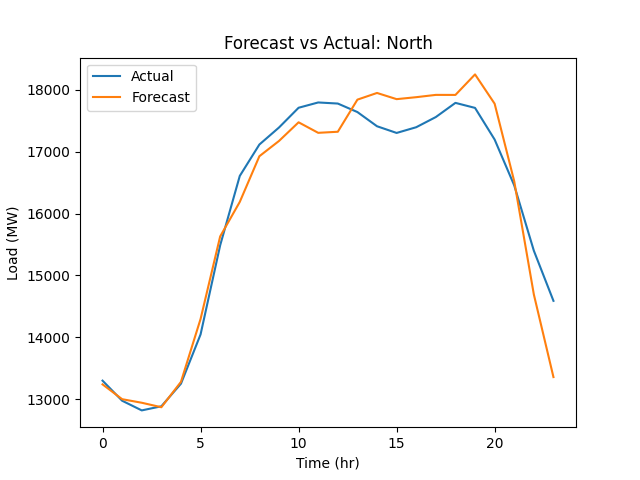
\includegraphics[width=0.9\linewidth]{load_forecast_north.png}
        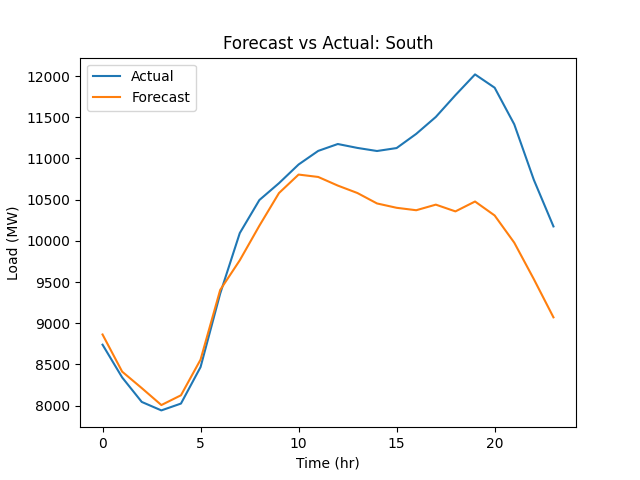
\includegraphics[width=0.9\linewidth]{load_forecast_south.png}
        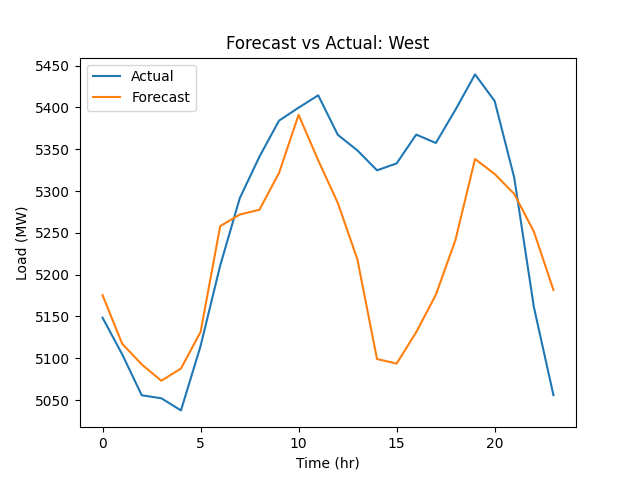
\includegraphics[width=0.9\linewidth]{load_forecast_west.png}
        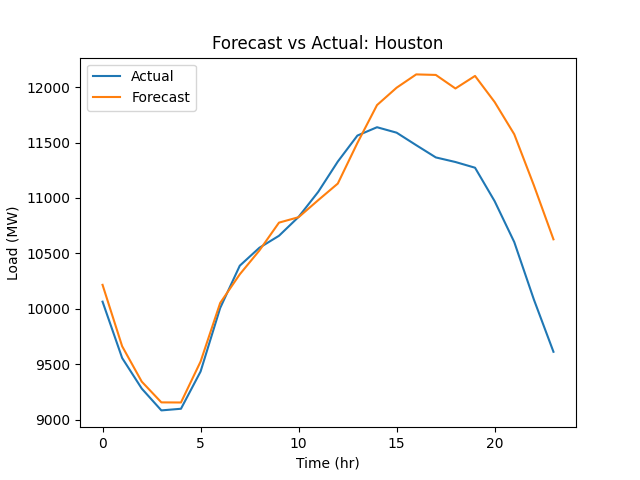
\includegraphics[width=0.9\linewidth]{load_forecast_houston.png}
    \end{center}

    For the total system, the error in the load expressed as a root mean square
    error is 2761.4 MW, and computed as mean average error is 10726.0 MW.
\end{letterenum}

\section{Distributed Solar PV}

\cite{razavi_impact_2019} reviews voltage regulation and system protection issues caused by distributed generation (DG)
and distributed PV,
within distribution systems. It also enumerates a number of solutions that have been proposed by
researchers. Key points include:

\begin{enumerate}
    \item Addition of PV to a distribution feeder changes the short-circuit levels which conflicts
        with the designed values of overcurrent relays, causing mis-operation of system protection
    \item Overcurrent relays can be replaced by directional overcurrent relays (DOCRs) to handle
        the reversal in power flow induced by DG.
    \item A number of adaptive protection schemes have been proposed by researchers to determine
        fault locations and optimize relay operating times within distribution systems containing DG.
    \item Voltage regulation issues are also caused by introduction of DG, as a result of bidirectional
        power flow.
    \item Conventional voltage regulation using e.g. on-load tap changers (OLTCs) can lead to voltage 
        stability issues in the presence of DG.
    \item Reactive power control within inverter-based DG units can help mitigate issues related to
        over-voltage.
\end{enumerate}


\section{Rate Design}
\begin{letterenum}
\item Rate design is important because it can act as a signal to improve communication and coordination
    between distributed energy resources (DERs). The design of rates, which are high during evening peaks
    and lower when during the day when solar resources are available, incentivizes customers to shift their
    energy usage away from peaks.

    Furthermore, if rates are communicated to at-home energy management systems (EMSs) in an automated manner, 
    then the EMS can automatically discharge stored battery power during peak times. This would allow
    owners of DERs to take full economic advantage of their energy storage investments by leveraging
    energy arbitrage oppurtunities, providing support to the grid in the process.

\item Again, designing energy costs to be high during the evening peaks incentivizes load shifting
    towards times when energy prices are cheaper. In terms of economic feasibility, a more evenly
    shaped load profile (in the case of conventional generation) or a load profile more closely aligned
    with renewable generation availability will reduce the costs of energy on the scale of the overall grid.
    Well-designed electricity rates would ideally share that economic benefit between residential consumers and
    the utility.

    The largest challenge of such a proposition is making the most economic solution readily
    convenient to the consumer. For example, if a customer's EV is designed to start charging as soon
    as it is plugged in, then to take advantage of the utility's rate design, the customer
    might need to walk into their garage to plug in the EV during the middle of the night. Clearly,
    this would be a major inconvenience, compliance would be low, and the overall influence of the designed
    rate upon the load profile would be small.

    On the other hand, an EV which is automatically capable of delaying its charging until off-peak hours
    would allow the customer to just plug in their EV when the get home and forget about it: much more convenient
    and likely to produce a significant shift in the load profile. This highlights the need for EMSs
    which can automatically take advantage of price differences to maximize the effectiveness of rate design.
\end{letterenum}

\bibliographystyle{plain}
\bibliography{RenEngHW}


\end{document}
